%%% Local Variables: 
%%% mode: latex
%%% TeX-master: t
%%% End:

\documentclass[a4paper, 10pt]{article}

\usepackage[utf8]{inputenc}
\usepackage{hyperref}
\usepackage{enumerate}
\usepackage{multirow}
\usepackage{wrapfig}

\usepackage{fancyvrb}
\DefineVerbatimEnvironment{code}{Verbatim}{fontsize=\small}
\DefineVerbatimEnvironment{example}{Verbatim}{fontsize=\small}

\usepackage{graphicx}
% \usepackage[margin=2cm]{geometry}
\usepackage[backend=bibtex]{biblatex}
\addbibresource{references.bib}

\title{Software Reengineering\\
       Assignment 2}
\author{Joey Ezechi\"{e}ls (1338994) \and Volker Lanting (1513273)}

% % Implement x.yy numbering scheme for subsections
% % where yy is *always* a 2-digit number
% \makeatletter
% \renewcommand\thesubsection{\thesection.\two@digits{\arabic{subsection}}}
% \makeatother

\begin{document}
\maketitle % Doesn't count towards the total number of pages
\pagenumbering{roman}

\newpage
\tableofcontents % Doesn't count towards the total number of pages

% \newpage
% \section{Introduction}
% \label{sec:introduction}

\newpage
\pagenumbering{arabic}
\section{Introduction}


% \newpage
\section{Elected reengineerings}
\label{sec:elected_reengineerings}
We have chosen to reengineer the following parts of the JME3 core code
base:
\begin{enumerate}
\item \textbf{JmeSystem}.
\end{enumerate}

% \newpage
\section{Motivation}
The reason we have chosen the various parts of the codebase (see
section \ref{sec:elected_reengineerings}) are as follows:
\begin{enumerate}
\item \textbf{JmeSystem} was chosen because it's not too large, it's
  a good example of a S.O.L.I.D. SRP violation and it doesn't have too
  many incoming dependencies, meaning pre-refactoring testability is
  higher than with e.g. god classes.
\end{enumerate}


% \newpage
\section{Feasibility}
Given the scope of the refactorings

% \newpage
\section{Before}
Before the start of our refactoring, there were only 12 unit tests.
None of which covered the code we planned on refactoring.


% \newpage
\section{After}
We have written 86 test cases in total for the classes JmeSystem, JmeSystemDelegate, JmeDesktopSystem and JmeAndroidSystem.
Together with the 12 testcases that already existed, the testsuite has 98 tests (see Figure~\ref{fig:num-tests}).
This figure shows that we have a single test case with an error.
We did that on purpose, as it exposes a bug in the JmeSystemDelegate, 
where an execution branch can never be visited (equals check of a lowercase string and "PowerPC", see Figure~\ref{fig:bug}).

The testsuite is pretty extensive with a line covering well in the 80\% for the classes under test (see Figures~\ref{fig:cov-core},~\ref{fig:cov-desktop}~and~\ref{fig:cov-android}).
Only JmeDesktopSystem was not covered properly at only 71\%. 
This was due to some missing classes in our project (the Jogl classes),
making it impossible to fully test the class. 
However, those non-covered parts (newContextJogl) are actually almost duplicates (supported by incode code duplicate findings) of pieces that are covered (newContextLwjgl).
So we are still confident that our testsuite suffices.

\begin{figure}
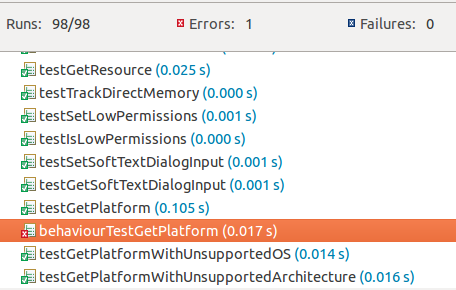
\includegraphics[width=\textwidth]{figures/86-new-tests.png}
\caption{a run of the test suite. Showing 98 testcases and a single failure (indicating the bug of Figure~\ref{fig:bug})}
\label{fig:num-tests}
\end{figure}

\begin{figure}
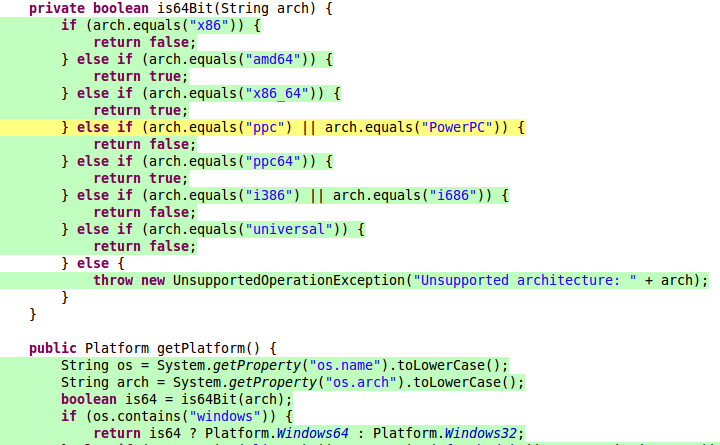
\includegraphics[width=\textwidth]{figures/bug-in-delegate.png}
\caption{The coverage indicates that the branch on matching "PowerPC" is not covered. The only call to is64 actually only passes lowercased strings.}
\label{fig:bug}
\end{figure}

\begin{figure}
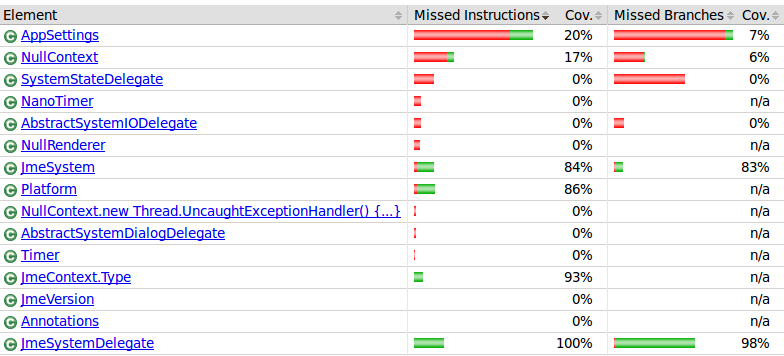
\includegraphics[width=\textwidth]{figures/test-coverage-core.png}
\caption{Test coverage for the com.jme3.system package in the src/core folder. We made testsuites for JmeSystem and JmeSystemDelegate.}
\label{fig:cov-core}
\end{figure}

\begin{figure}
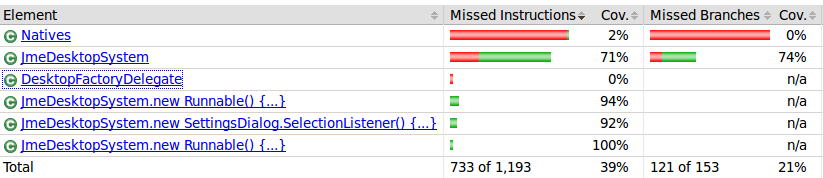
\includegraphics[width=\textwidth]{figures/test-coverage-desktop.png}
\caption{Test coverage for the com.jme3.system package in the src/desktop folder. We made a testsuite for JmeDesktopSystem.}
\label{fig:cov-desktop}
\end{figure}

\begin{figure}
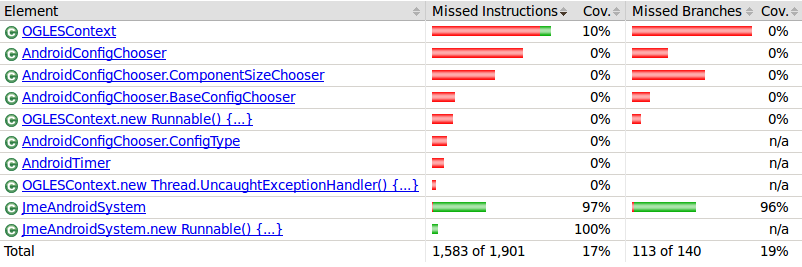
\includegraphics[width=\textwidth]{figures/test-coverage-android.png}
\caption{Test coverage for the com.jme3.system.android package in the src/android folder. We made a testsuite for JmeAndroidSystem.}
\label{fig:cov-android}
\end{figure}

\end{document}
